\documentclass[12pt]{article}
\usepackage[utf8]{inputenc}
\usepackage[T2A]{fontenc}
\usepackage[mongolian]{babel}
\usepackage{graphicx}
\graphicspath{{Image}}
\title{Санал асуулга}
\begin{document}
\section{Функционал шаардлага}
 Энэхүү модуль нь сурагч, багш, сургалтын алба гэсэн 3-н оролцогчтой.
Сурагчийн функциональ шаардлага:
\begin{enumerate}
	\item Багш болон сургалтын албаны явуулж буй санал асуулгад санал өгөх
	\item Санал асуулгын үр дүнг харах(санал оруулагч үр дүнг харах боломжтойгоор тохируулсан тохиолдолд)
	\item Өөрийн ангийн хүүхдүүдээс санал асуулга авах
	\item Явуулсан санал асуулгынхаа дүнг харах
\end{enumerate}
Багшийн функциональ шаардлага:
\begin{enumerate}
	\item Хичээл заадаг нийт хүүхдүүдээс санал асуулга авах
	\item Хичээл заадаг анги сонгон санал асуулга авах
	\item Сургалтын албанаас явуулж буй санал асуулгад санал өгөх(өгөх эрхтэй бол)
	\item Санал асуулгын үр дүнг харах(санал оруулагч үр дүнг харах боломжтойгоор тохируулсан тохиолдолд)
	\item Явуулсан санал асуулгынхаа дүнг харах 
\end{enumerate}
Сургалтын албаны функциональ шаардлага
\begin{enumerate}
	\item Нийт гагш нараас санал асуулга авах
	\item Нийт сурагчдаас санал асуулга авах
	\item Тэнхимээр зааглан нийт багш эсвэл сурагчдаас санал асуулга авах
	\item Явуулсан санал асуулгынхаа дүнг харах
	\end{enumerate}
\section{Функционал бус шаардлага}
\begin{enumerate}
	\item Систем нь хүнд ойлгомжтой загвартай байх
	\item Нэг хүн нэгээс олон санал өгөх, санал асуулга эхлэх өдрөөс өмнө эсвэл төгсөх өдрөөс хойш санал өгөх зэргээс систем хамгаалагдсан байх
	\item Эрхээр тусгаарлагдсан байх
\end{enumerate}
 	\section{Юзкэйс диаграм}
		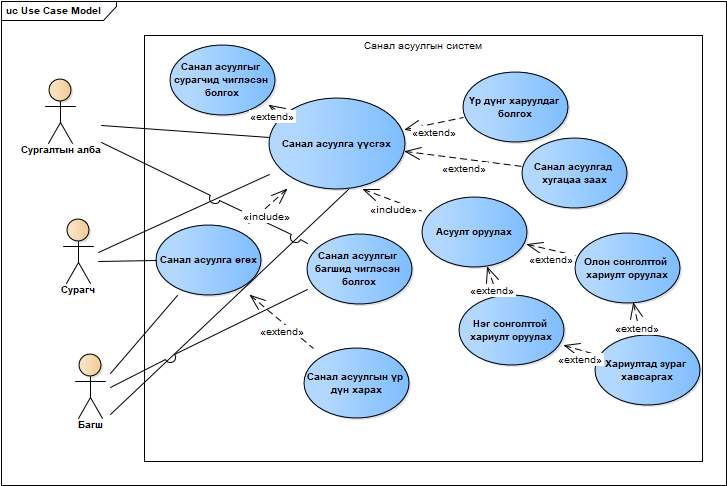
\includegraphics[scale=0.6]{usecase}
	\section{Класс диаграм}
		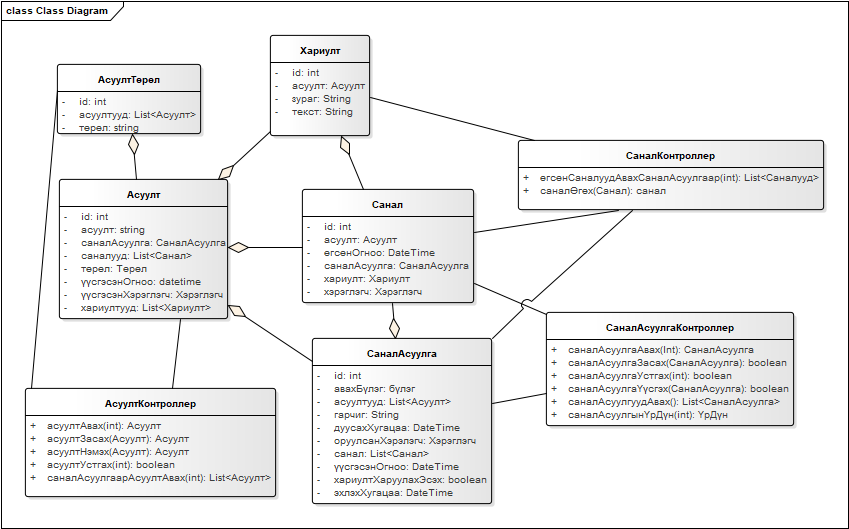
\includegraphics[angle=90,scale=0.6]{class_diagram}
	\end{document}
 